
\documentclass{sigplanconf}

% The following \documentclass options may be useful:

% preprint      Remove this option only once the paper is in final form.
% 10pt          To set in 10-point type instead of 9-point.
% 11pt          To set in 11-point type instead of 9-point.
% authoryear    To obtain author/year citation style instead of numeric.
\synctex=-1

\usepackage[utf8]{inputenc}
\usepackage{array}
\usepackage{color}
\usepackage{amsmath}
\usepackage{amssymb}
\usepackage{fixltx2e}
\usepackage{graphicx}
\usepackage[unicode=true,pdfusetitle,
 bookmarks=true,bookmarksnumbered=false,bookmarksopen=false,
 breaklinks=false,pdfborder={0 0 1},backref=false,colorlinks=false]{hyperref}


\makeatletter
\usepackage{enumitem}
\usepackage{multicol}
\usepackage{tabularx}

%%%%%%%%%%%%%%%%%%%%%%%%%%%%%% LyX specific LaTeX commands.
\usepackage{float}
\floatstyle{ruled}
\newfloat{code}{tbp}{loa}
\providecommand{\codename}{Listing}
\floatname{code}{\protect\codename}


% nice listings
\usepackage{xcolor}
\usepackage{newverbs}

\usepackage{color}
\definecolor{verylightgray}{rgb}{0.93,0.93,0.93}
\definecolor{darkblue}{rgb}{0.2,0.2,0.6}
\definecolor{commentgreen}{rgb}{0.25,0.5,0.37}
\usepackage{letltxmacro}

\usepackage{listings}

\makeatletter
\LetLtxMacro{\oldlstinline}{\lstinline}

\renewcommand\lstinline[1][]{%
  \Collectverb{\@@myverb}%
}

\def\@@myverb#1{%
    \begingroup
    \fboxsep=0.2em
    \colorbox{verylightgray}{\oldlstinline|#1|}%
    \endgroup
}
\makeatother




\lstset{backgroundcolor={\color{verylightgray}},
  basicstyle={\scriptsize\ttfamily},
  commentstyle={\ttfamily\color{commentgreen}},
  keywordstyle={\bfseries\color{darkblue}},
  morecomment={[l]{//}},
  tabsize=4,
  morekeywords={foreach,in,def,type,dynamic,Int,
    Boolean,infer,void,super,if,boolean,int,else,
    while,do,extends,class,assert,for,switch,case,
    private,protected,public,const,final,static,
    interface,new,true,false,null,return}}
\renewcommand{\lstlistingname}{Listing}



\newcommand{\mynote}[2]{%
  \textcolor{red}{%
    \fbox{\bfseries\sffamily\scriptsize#1}%
    {\small$\blacktriangleright$\textsf{\emph{#2}}$\blacktriangleleft$}%
  }%
}

\newcommand\remi[1]{\mynote{Remi}{#1}}
\newcommand\cfbolz[1]{\mynote{cfbolz}{#1}}
\newcommand\arigo[1]{\mynote{arigo}{#1}}



\begin{document}

\special{papersize=8.5in,11in}
\setlength{\pdfpageheight}{\paperheight}
\setlength{\pdfpagewidth}{\paperwidth}

\conferenceinfo{DLS 2014}{to be supplied}
\copyrightyear{2014}
%\copyrightdata{978-1-nnnn-nnnn-n/yy/mm}
\doi{nnnnnnn.nnnnnnn}

% Uncomment one of the following two, if you are not going for the
% traditional copyright transfer agreement.

%\exclusivelicense                % ACM gets exclusive license to publish,
                                  % you retain copyright

%\permissiontopublish             % ACM gets nonexclusive license to publish
                                  % (paid open-access papers,
                                  % short abstracts)

%% \titlebanner{banner above paper title}        % These are ignored unless
%% \preprintfooter{short description of paper}   % 'preprint' option specified.

\title{Virtual Memory Assisted Transactional Memory for Dynamic Languages}
\subtitle{DLS'14}

\authorinfo{Remigius Meier}
           {Department of Computer Science\\ ETH Zürich}
           {remi.meier@inf.ethz.ch}
\authorinfo{Armin Rigo}
           {www.pypy.org}
           {arigo@tunes.org}

\maketitle

\begin{abstract}
....
\end{abstract}

%\category{CR-number}{subcategory}{third-level}

% general terms are not compulsory anymore,
% you may leave them out
%% \terms
%% term1, term2

\keywords
...

\section{Introduction}


Dynamic languages like Python, PHP, Ruby, and JavaScript are usually
regarded as very expressive but also very slow. In recent years, the
introduction of just-in-time compilers (JIT) for these languages
(e.g.\ PyPy~\cite{cfbolz09}, V8~\cite{kevin10}, IonMonkey~\cite{ionmonkey})
started to change this perception by delivering
good performance that enables new applications. However, a parallel
programming model was not part of the design of those languages. Thus,
the reference implementations of e.g.\ Python and Ruby use a single,
global interpreter lock (GIL) to serialise the execution of code in
threads.

While this GIL prevents any parallelism from occurring, it also
provides some useful guarantees. Since this lock is always acquired
while executing bytecode instructions and it may only be released
in-between such instructions, it provides perfect isolation and
atomicity between multiple threads for a series of
instructions. Additionally, it provides the application with a
sequential consistency model~\cite{lamport79}. Another technology that
can provide the same guarantees is transactional memory (TM).

There have been several attempts at replacing the GIL with
TM~\cite{nicholas06,odaira14,fuad10}. Using transactions to enclose
multiple bytecode instructions, we can get the very same semantics as
the GIL while possibly executing several transactions in
parallel. Furthermore, by exposing these interpreter-level
transactions to the application in the form of \emph{atomic
blocks}~\cite{tim03,tim05}, we give dynamic languages a new
synchronisation mechanism that avoids several of the problems of locks
as they are used now.

TM systems can be broadly categorised as hardware based (HTM),
software based (STM), or hybrid systems (HyTM). HTM systems are limited
by hardware constraints~\cite{odaira14,fuad10}, while STM systems have
a lot of overhead~\cite{cascaval08,drago11}. In~\cite{wayforward14},
we argue that STM is still the best way forward, especially since it
supports large atomic blocks as a new way for synchronising multiple
threads. There have been several attempts at lowering the overhead
of STM~\cite{warmhoff13,spear09} -- sometimes at the cost of scalability.
In this paper, we describe how we manage to lower the overhead of our
STM system so that it can be seen as a viable replacement for the GIL.

\cfbolz{both the introduction and the contributions need to stress the co-design of GC and STM}

Our contributions include:
\begin{itemize}[noitemsep]
\item We introduce a new software transactional memory (STM) system
  that performs well on low numbers of CPUs.
\item We make novel use of the memory management capabilities of
  off-the-shelf CPUs, e.g. memory segmentation and 64bit address space.
\item We integrate our STM system closely with a garbage collector
  (GC) in order to lower the overhead of STM.
\item This new STM system is used to replace the GIL in one
  implementation of Python and is then evaluated extensively.
\item We introduce atomic blocks to the Python language to provide a
  backwards compatible, composable synchronisation mechanism for
  threads.
\end{itemize}



\section{Background}

\subsection{Global Interpreter Lock}

The GIL is a very simple synchronisation mechanism for supporting
multithreading in an interpreter. The basic guarantee is that the GIL
may only be released in between bytecode instructions. Thus, these
instructions are always executed atomically and in complete isolation
from others running in other threads. \emph{Atomicity} means that each
instruction and its effects seem to happen at one, indivisible point
in time. Other instructions never see inconsistent state of a
partially executed instruction (\emph{isolation}).

In addition to these guarantees, instructions are executed in a
sequential consistency model~\cite{lamport79}. This means that
the outcome of any execution of instructions in multiple threads is
equal to \emph{some} sequential execution of them.


\subsection{Transactional Memory}

Transactional memory (TM) is a concurrency control mechanism that
comes from database systems. Using transactions, we can group a series
of instructions performing operations on memory and make them happen
atomically and in complete isolation from other transactions.
Atomicity and isolation are basic properties of transactions.

If we start multiple such transactions in multiple threads, the TM
system guarantees that the outcome of running the transactions is
\emph{serialisable}. Meaning, the outcome is equal to some sequential
execution of these transactions. By that, we can again provide a
sequentially consistent model for programming in multiple threads. We
can therefore use TM to directly replace the GIL. Instead of releasing
and acquiring the GIL between bytecode instructions, we commit and
start the transactions our instructions are running in.

\subsection{Python}

We implement and evaluate our system for the Python language. Python
is a dynamic programming language that was designed with GIL semantics
in mind. Its reference implementation, CPython~\cite{cpython}, uses a
GIL to synchronise instructions in multiple threads.
Over the years, Python added multiple ways to provide concurrency and
parallelism to its applications. We want to highlight two of them,
namely \emph{threading} and \emph{multiprocessing}.

\emph{Threading} employs operating system (OS) threads to provide
concurrency. It is, however, limited by the GIL and thus does not
provide parallelism. At this point we should mention that it is indeed
possible to run external functions written in C instead of Python in
parallel. Our work focuses on Python itself and ignores this aspect as
it requires writing in a different language.

The second approach, \emph{multiprocessing}, uses multiple instances
of the interpreter itself and runs them in separate OS processes.
Here we actually get parallelism because we have one GIL per
interpreter, but of course we have the overhead of multiple processes~/
interpreters and also need to exchange data between them explicitly
and expensively.

We focus on the \emph{threading} approach. This requires us to remove
the GIL from our interpreter in order to run code in parallel on
multiple threads. One approach to this is fine-grained locking instead
of a single global lock. Jython~\cite{webjython} and
IronPython~\cite{ironpython} are implementations of this. It requires
great care in order to avoid deadlocks, which is why we follow the TM
approach that provides a \emph{direct} replacement for the GIL. It
does not require careful placing of locks in the right spots.


\subsection{Synchronisation}

In Python, since the GIL is not directly exposed to the interpreter,
applications still need to synchronise memory accesses from multiple
threads using locks. Locks can be very hard to get
right~\cite{christopher10,victor11,shan08}.  They are non-composable,
have overhead, may deadlock, limit scalability, and add to the overall
complexity of the program logic. We think that \emph{atomic
blocks}~\cite{tim03,tim05} provide a better way for synchronisation.

Atomic blocks are composable, deadlock-free, higher-level and expose
useful atomicity and isolation guarantees to the application for a
series of instructions. This is why we think that the introduction
of atomic blocks to Python is a valuable contribution. Since atomicity
is a property of transactions, TM and atomic blocks are a natural fit.



\section{Transactional Memory Model}

In this section, we characterise the model of our TM system and its
guarantees as well as some of the design choices we made. This should
clarify the general semantics in commonly used terms from the
literature~\cite{harris10}.

Our TM system is fully implemented in software. However, we do exploit
some more advanced features of current CPUs, particularly \emph{memory
segmentation, virtual memory,} and the 64-bit address space. Still,
it cannot be classified as a hybrid TM system since it currently
makes no use of any HTM present in the CPU.

\subsection{Conflict Handling}

We implement an object-based TM system, thus it makes sense to detect
conflicts with \emph{object granularity}. With this choice, if two
transactions access the same object and at least one access is a
write, we count it as a conflict. Conceptually, it is based on
\emph{read} and \emph{write sets} of transactions. Reading from an
object adds the object to the read set, writing to it adds it to both
sets. Two transactions conflict if they have accessed a common object
that is in the write set of at least one of them.

The detection, or \emph{concurrency control}, works partly
\emph{optimistically} for reading objects. Read-write conflicts
between two transactions are detected in both exactly at the time when
the writing one commits. For write-write conflicts we are currently
\emph{pessimistic}: Only one transaction may have a certain object in
its write set at any point in time, others trying to write to it will
have to wait or abort. This decision needs to be evaluated further
in the future.

When a conflict is detected, we perform some simple contention
management that generally prefers the older transaction to the younger.

\subsection{Semantics}

As required for TM systems, we guarantee complete \emph{isolation} and
\emph{atomicity} for transactions at all times. Our method of choice
is \emph{lazy version management}. Modifications by a transaction are
not visible to another transaction before the former commits.
Furthermore, the isolation provides full
\emph{opacity}~\cite{guerraoui08} to always guarantee a consistent
read set even for non-committed transactions.

To also support these properties for irreversible operations that
cannot be undone when we abort a transaction (e.g.\ I/O, syscalls, and
non-transactional code in general), we use \emph{irrevocable} or
\emph{inevitable transactions}~\cite{blundell06,spear08}. These transactions are always
guaranteed to commit, which is why they always have to win in case
there is a conflict with another, normal transaction. There is always
at most one such transaction running in the system, thus their
execution is serialised. With this guarantee, providing \emph{strong
isolation} and \emph{serialisability} between non-transactional code
is possible by making the current transaction inevitable right before
running irreversible operations.



\section{High-level overview}

In this section, we will present the general idea of how the TM model is
implemented.  The later section~\ref{sub:Low-level-Implementation} will
discuss it with more technical details.

\subsection{Memory Segmentation and Page Sharing}

A naive approach to providing complete isolation between threads is to
partition the virtual memory of a process into $N$ segments, one per
thread.  Each segment then holds a complete copy of the memory logically
seen by the program.  All threads read and write data inside their own
segment; exchanges between segments occur only at commit-time.  So far,
this is a model that would also work for distributed transactional
memory.

Obviously, if we are in a shared-memory setting, this model is extremely
wasteful: at a given time, most objects are identical in all, or most,
segments.  They differ only in segments that have modified but not yet
committed the object.  So we use a trick of the Memory Management Unit
(MMU) of the CPU.  At the coarse unit of one page of memory (4096
bytes), we use remappings so that, in general, pages within segments are
\emph{shared} with each other if they would contain a fully identical
copy.  Conversely, when one segment needs to write to one object
contained in a page, the complete page is first \emph{privatised:} it is
duplicated and the copy is remapped so that it will be visible in this
segment (only).  This process is illustrated in
Figure~\ref{fig:Page-Remapping}.

The result that we get is that the virtual address space of the process
is bloated -- by a factor $N$ -- but the real memory usage is not --
because most pages are shared with their copies in most other segments.

\begin{figure}[h]
  \centering
  \includegraphics[width=1\columnwidth]{\string"page remapping\string".pdf}
  \caption{Page Remapping: (I) initial setting. (II) remap all pages to
    segment~0, fully shared memory configuration. (III) privatise single
    pages.\label{fig:Page-Remapping}}
\end{figure}


\subsection{Memory Segmentation on the x86}

When we need to store into our objects pointers to other objects, we
need to be careful: if we were to directly store regular addresses valid
in the local segment, then the objects' binary content would have to differ
between segments.  This would prevent any sharing.  Instead, we store
pointers as \emph{Segment Offsets ($SO$)}, i.e.\ offsets from the start
of the segment.  A $SO$ can then be interpreted from any segment by
adding it to the base address of that segment.\footnote{An alternative
model would be to simulate threads using several independent processes
in which all segments are at the same address.  This might work well for
demonstration purposes, but it is not really suitable for implementing
an existing programming language: programs assume that most of the state
(file descriptors, external libraries, ...) is shared.} The result is
called a \emph{Linear Address (LA)}. This is illustrated in
Figure~\ref{fig:Segment-Addressing}.

The x86 CPUs provide a feature which is precisely called \emph{memory
segmentation}.  On the modern x86-64, this is enough to perform the
addition described above very efficiently.  We use the segment register
$\%gs$, which is available to applications, to point to the
thread's segment start address.\footnote{The other segment register
$\%fs$ is typically used by the threading library to provide access to
thread-local data.  One point of view is that we are using $\%gs$ for a
similar purpose: thread-local data -- but a lot of it.}  The translation
from a $SO$ to a LA is done for us by using the ``$\%gs\colon$'' prefix
before any CPU instruction that reads or writes memory using a $SO$
address.  This is very efficient and some compilers support it natively
(e.g.\ clang).

If support for this is not available (due to the compiler or on a
different architecture), there are other optimizations possible.  For
example, using gcc, a regular register can be globally reserved and
all ``simple enough'' memory accesses will still resolve to a single
instruction.  More complicated accesses, e.g.\ those involving array
indexing, will need an extra explicit addition.

\begin{figure*}[t]
  \centering
  \includegraphics[scale=0.8]{\string"segment addressing\string".pdf}
  \caption{Segment Addressing\label{fig:Segment-Addressing}}
\end{figure*}


\subsection{Conflict detection}

What we described so far has no mesurable performance impact by itself,
but is missing conflict detection to be part of a full-fledged STM
system.  This requires adding \emph{barriers} to the program to register
the objects into the read or write set, and adapting the commit
protocol in consequence.

\begin{description}

\item [{Read~Barrier:}] A major contribution to our performance results
  is the simplicity of the read barrier: a large program (like an
  interpreter for a complex language) contains a number of reads that
  typically exceeds many times the number of writes.  We managed to
  design the read barrier so that it is done by one memory write
  (setting a flag) into non-shared memory.  This is done with a
  segment-local array of flags indexed by a number derived from the $SO$
  of the object.  Unlike other STM systems, the read barrier does not
  have to find the private version of some object -- our two-step
  address translation automatically resolves the reference to the
  private version on every access anyway.  This means the read barrier
  is not constrained to execute before the actual read -- both the
  compiler and the CPU are free to reorder them.

\item [{Write~Barrier:}] This is triggered by checking a flag in the
  header of the object.  When the flag is set, we call the slow path,
  which adds the object into the write set and unconditionally resets
  the flag.  We eagerly detect write-write conflicts by allowing only
  one transaction modifying an object at a time (by acquiring a write
  lock).\footnote{Eager write-write detection is not inherent to our
  approach; future experiments may show that we want to lift this
  restriction.}  This slow path is also responsible for privatising
  pages,\footnote{The write set contains objects, not pages.} as
  described above.  Interestingly, we are using a generational garbage
  collector (described below) which requires a similar write barrier
  anyway -- so the same header flag is used for both cases.  The flag
  means ``something needs to be done before writing to this object'',
  and the slow path logic determines what it is.

\item [{Commit:}] When we want to commit a transaction, we need to check
  for read-write conflicts.  Such conflicts cannot be detected in the
  minimal read barrier, but can be detected during commit: the case to
  look for is that the committing transaction wrote to an object that
  another transaction has already read.\footnote{Which is why the read
  sets can be just sparsely populated arrays of flags: we never walk the
  whole read set.} A priori, checking other transactions' read sets
  would involve reading concurrently modified memory: a different thread
  could be issuing a read barrier in parallel with an unprotected
  commit.  To prevent this from occurring, we must suspend all other
  threads at known safe points.  This is a trade-off for the simplicity
  of our read barriers -- which is well worth it in our case, due to the
  very high number of read barriers when compared to the number of
  commits and the (low) total number of threads.

\end{description}

Conflicts can be resolved by aborting one of the two transactions, or in
some cases by pausing one of them until the other commits.  If a commit
succeeds, we copy the changes to modified objects so that they become
visible in other segments.  Note that this only includes objects that
existed before the transaction and have been modified by it.  It does
not include all the new objects created by the current transaction
(there is typically a very high rate of object churn in dynamic languages).
Our garbage collector allocates new objects in pages that are shared in
the first place, so that they do not need to be copied -- and moreover,
such objects will commonly never be modified any more.

Privatised pages are re-shared during major collection cycles.



\section{Low-level Implementation\label{sub:Low-level-Implementation}}

In this section, we will provide details about the actual
implementation of the system and discuss some of the issues that we
encountered.


\subsection{Architecture}

Our TM system is designed as a library that covers all aspects around
transactions and object management. It is designed for object-oriented
dynamic language VMs as a replacement for the GIL.

The library consists of two parts: (I) It provides a simple interface
to starting and committing transactions, as well as the required read
and write barriers. (II) It also includes a \emph{garbage collector
(GC)} that is closely integrated with the TM part (e.g.\ it shares the
write barrier). The close integration helps in order to know more
about the lifetime of an object, as will be explained in the following
sections.


\subsection{Application Programming Interface\label{sub:Application-Programming-Interfac}}

\begin{lstlisting}
void stm_start_transaction()
void stm_commit_transaction()
void stm_read(object_t *SO)
void stm_write(object_t *SO)
object_t *stm_allocate(ssize_t size_rounded)
STM_PUSH_ROOT(object_t *SO)
STM_POP_ROOT(object_t *SO)
\end{lstlisting}


\lstinline!stm_start_transaction()!  starts a transaction in the
current thread. Internally, it uses \lstinline!setjmp()! to remember
where the transaction started in case of an abort.
\lstinline!stm_commit_transaction()! tries to commit the current
transaction. \lstinline!stm_read()!, \lstinline!stm_write()!  perform
a read or a write barrier on the object given as the argument, and
\lstinline!stm_allocate()!  allocates a new object with the specified
size.  \lstinline!STM_PUSH_ROOT()! and \lstinline!STM_POP_ROOT()!
push and pop objects onto the shadow stack\footnote{A stack for pointers
  to GC objects that allows for precise garbage collection. All objects
  on that stack are never seen as garbage and are thus always kept
  alive.~\cite{fergus02}} of the current thread.  References to objects
have to be saved using this stack around calls that may cause a GC
cycle to happen, and also while there is no transaction
running. Otherwise these references may not be valid any more because
the object moved or was seen as garbage. In this simplified API, only
\lstinline!stm_allocate()!  and \lstinline!stm_commit_transaction()!
require saving object references.

In the following sections, whenever we use $SO$, we go through the
address translation to get to the actual contents of an object. This
is also signified by the type \lstinline!object_t!.  This type is
special as it causes the
compiler\footnote{We use Clang 3.5 with patches to deal with bugs in
its ``address-space 256'' feature. Patches are available from authors
until inclusion into the official clang.} to make all accesses through
it relative to the $\%gs$ register.  With exceptions, nearly all
accesses to objects managed by the TM system should use this type so
that the CPU will translate the reference to the right version of the
object.


\medskip   % why, Latex, why??
\subsection{Setup\label{sub:Setup}}

On startup, we reserve a big range of virtual memory with a call to
\lstinline!mmap()! and partition this space into $N+1$ segments. We
want to run $N$ threads in parallel while segment~0 is designated as
the \emph{sharing-segment} that is never assigned to a thread. The
sharing-segment is essentially read-only except during commit.

The next step involves using \lstinline!remap_file_pages()!, a Linux
system call\footnote{remap\_file\_pages() can also be done with more mmap()
calls in a roughly portable way, but the former is more efficient on Linux.},
to establish the \emph{fully-shared configuration}.  All pages
of segments $>0$ map to the pages of the sharing-segment.

However, the layout of a segment is not uniform and we actually
privatise a few areas again right away. These areas are illustrated in
Figure~\ref{fig:Segment-Layout} and explained here:
\begin{description}[noitemsep]
\item [{NULL~page:}] This page is unmapped and will produce a
  segmentation violation when accessed. We use this to detect
  erroneous dereferencing of \lstinline!NULL! references.  All
  $\%gs{::}SO$ translated to linear addresses will point to NULL pages
  if $SO$ is set to \lstinline!NULL!.
\item [{Segment-local~data:}] Some area private to the segment that
  contains segment-local information.
\item [{Read~markers:}] These are pages that store information about
  which objects were read in the current transaction running in this
  segment.
\item [{Nursery:}] This area contains all the freshly allocated
  objects (\emph{young objects}) of the current transaction. The GC
  uses bump-pointer allocation in this area to allocate objects in the
  first generation.
\item [{Old~object~space:}] These pages are the ones that are really
  shared between segments. They mostly contain old objects but also
  some young ones that were too big to be allocated in the nursery.
\end{description}



\begin{figure*}[t]
  \centering
  \includegraphics[scale=0.8]{\string"segment layout\string".pdf}
  \caption{Segment Layout\label{fig:Segment-Layout}}
\end{figure*}



\subsection{Assigning Segments}

From the above setup it is clear that the number of segments is
statically set to some $N$. That means that at any point in time, a
maximum of $N$ threads and their transactions can be running in
parallel.  To support an unlimited number of threads in applications
that use this TM system, we assign segments dynamically to threads.

At the start of a transaction, the thread it is running in acquires a
segment. It may have to wait until another thread finishes its
transaction and releases a segment. Fairness is not guaranteed yet, as
we simply assume a fair scheduling policy in the operating system when
waiting on a condition variable.

Therefore, a thread may be assigned to different segments each time it
starts a transaction. Although, we try to assign it the same segment
again if possible.




\subsection{Garbage Collection}

Garbage collection plays a big role in our TM system. The GC is
generational and has two generations: the \emph{young} and the
\emph{old} generation. It is optimised for dynamic languages with
high allocation rates.

The \textbf{young generation}, where objects are considered to be
\emph{young} and reside in the \emph{Nursery}, is collected by
\emph{minor collections}. These collections move the surviving objects
out of a thread's nursery into the old object space, which can be done
without stopping other threads. This is happens either if the nursery has
no space left anymore or if we are committing the current
transaction. Consequently, all objects are old and the nursery empty
after a transaction commits.  Furthermore, all objects in the nursery
were always created in the current transaction. This fact is useful
since we do not need to call any barrier on this kind of objects.

To improve this situation even more, we introduce the concept of
\emph{overflow objects}. If a minor collection needs to occur during a
transaction, we empty the nursery and mark each surviving object in
the old object space with an \lstinline!overflow_number!  globally
unique to the current transaction. That way we can still detect in a
medium-fast path inside barriers that the object still belongs to the
current transaction. \remi{so this is where we mention how the GC-STM
integration is useful. highlight more or move to own section?}
\cfbolz{definitely its own section listing all the benefits}

The \textbf{old generation}, where objects are considered to be
\emph{old} and never move again, is collected by \emph{major
  collections}.  These collections are implemented in a stop-the-world
kind of way and first force minor collections in all threads. The
major goal is to free objects in the old objects space. Furthermore,
we optimistically re-share pages that do not need to be private
anymore.

As seen in the API (section~\ref{sub:Application-Programming-Interfac}),
we use a \emph{shadow stack}~\cite{fergus02} in order to provide precise garbage
collection.  Any time we call a function that possibly triggers a
collection, we need to save the objects that we need afterwards on the
shadow stack using \lstinline!STM_PUSH_ROOT()!.  That way, they will
not be freed. And in case they were young, we get their new location
in the old object space when getting them back from the stack using
\lstinline!STM_POP_ROOT()!.




\subsection{Read Barrier}

The point of the read barrier is to add the object to the read set of
the transaction. This information is needed to detect conflicts
between transactions. In other STM systems, it also resolves an object reference to
a private copy, but since the CPU performs our address translation on
every object access efficiently, we do not need to do that in our
barrier.

To add the object to the read set, for us it is enough to mark it as
read. Since this information needs to be local to the segment, we need
to store it in private pages. The area is called \emph{read markers}
and already mentioned in Section~\ref{sub:Setup}.

This area can be seen as a continuous, segment-local array of bytes
that is indexed with an object's reference ($SO$) divided by 16. So
that each object has its own read marker, all objects have a size of
at least 16 bytes. Otherwise there would be false conflicts when
reading from two adjacent objects that share a single marker.
Instead of just setting the byte to \lstinline!true!  if the
corresponding object was read, we set it to a \lstinline!read_version!
belonging to the transaction, which will be incremented on each
commit.  Thereby, we can avoid resetting the bytes to
\lstinline!false!  on commit and only need to do this every 255
transactions. The whole code for the barrier is easily optimisable for
compilers as well as perfectly predictable for CPUs:

\begin{lstlisting}
void stm_read(SO):
    *(SO >> 4) = read_version
\end{lstlisting}


\begin{figure}[h]
  \centering
  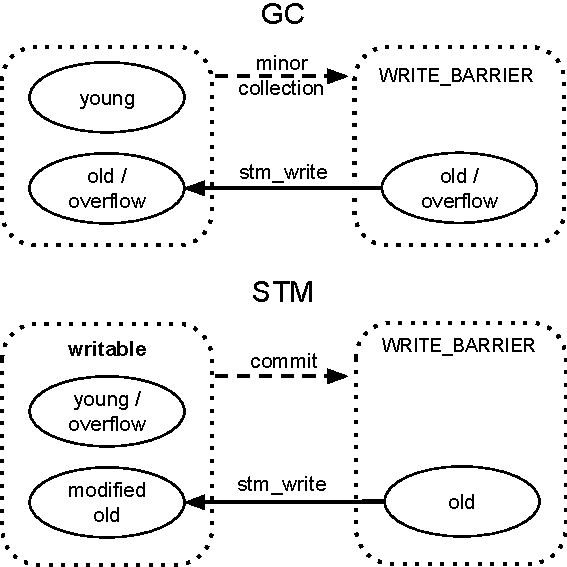
\includegraphics[width=1\columnwidth]{object_states.pdf}
  \caption{Objects states handled by the write barrier\label{fig:obj_states}}
\end{figure}


\subsection{Write Barrier}

The job of the write barrier is twofold: first, it serves as a write
barrier for the garbage collector and second, it supports COW and adds
objects to the write set of the transaction. These two jobs are
depicted in Figure~\ref{fig:obj_states}.

The \textbf{fast path} of the write barrier is very simple. We only
need to check for the flag \lstinline!WRITE_BARRIER! in the object's
header through its $SO$ and call the slow path if it is set. This flag
is set either if the object is old and comes from an earlier
transaction, or if there was a minor collection which will add the
flag again on all objects and may produce overflow objects. The flag
is never set on freshly allocated objects, because they do not need
to be traced by the GC or handled by the STM system. This fast path
covers all cases for the GC and for the STM system.


\begin{lstlisting}
void stm_write(SO):
	if SO->flags & WRITE_BARRIER:
		write_slowpath(SO)
\end{lstlisting}

\begin{code}[h]
\begin{lstlisting}
void write_slowpath(SO):
	// GC part:
	list_append(to_trace, SO)
	if is_overflow_obj(SO):
		SO->flags &= ~WRITE_BARRIER
		return
	// STM part
	stm_read(SO)
	lock_idx = SO >> 4
  retry:
	if write_locks[lock_idx] == our_num:
		// we already own it
	else if write_locks[lock_idx] == 0:
		if cmp_and_swap(&write_locks[lock_idx],
					    0, our_num):
			list_append(modified_old_objects, SO)
			privatize_pages(SO)
		else:
			goto retry
	else:
		w_w_contention_management()
		goto retry
	SO->flags &= ~WRITE_BARRIER
\end{lstlisting}

\caption{Slow path of the write barrier\label{lst:w_slow}}
\end{code}


The \textbf{slow path} is shown in Listing~\ref{lst:w_slow}.
First comes the \emph{GC part}: In any case, the object will be added
to the list of objects that need tracing in the next minor collection
(\lstinline!to_trace!).  This is necessary in case we write a
reference to it that points to a young object. We then need to trace
it during the next minor collection in order to mark the young object
alive and to update its reference to the new location it gets moved
to.

The check for \lstinline!is_overflow_obj()! looks at the
\lstinline!overflow_number!  and tells us if the object was actually
created in this transaction. In that case, we do not need to execute
the following \emph{STM part}.  We especially do not need to privatise
its pages since no other transaction knows about these overflow
objects. Even if they reside in non-private pages, it is guaranteed
that no other transaction can have a reference to them.

Up to here, we see that all cases of the GC shown in
Figure~\ref{fig:obj_states} are handled. What is left is to handle the
cases of the STM system that need to make old objects writable.

For the \emph{STM part}, we first perform a read barrier on the
object. We then try to acquire its write lock. \lstinline!write_locks!
is a simple, \textbf{global} array of bytes that is indexed with the
$SO$ of the object divided by 16. Note, ``global'' here really means
it is a single array with data for all segments, there is no address
translation going on to access its elements contrary to e.g.\ the
read markers array.  If we already own the lock, we are done.
If someone else owns the lock, we will do a write-write contention
management that will abort either us or the current owner of the
object.  If we succeed in acquiring the lock using an atomic
\lstinline!cmp_and_swap!, we need to add the object to the write set
(a simple list called \lstinline!modified_old_objects!)  and privatise
all pages belonging to it (copy-on-write).

In all cases, we remove the \lstinline!WRITE_BARRIER!  flag from the
object before we return. Thus, we never trigger the slow path again
before we do the next minor collection or we start the next
transaction.\footnote{We always do a minor collection during a commit.}

Note that we have three kinds of objects: \emph{young, overflow} and
\emph{old} objects. Young and overflow objects were created in the
same transaction; old objects always come from previous transactions.
The close integration between STM and the GC allows us to use this
information effectively: young objects do not trigger the slow path at
all, overflow objects only need to be handled by the GC part of the
write barrier once between collections, and only the old objects need
to be handled by the TM part once per transaction. This keeps the
overhead of the write barrier very low.


\subsection{Abort}

Aborting a transaction is rather easy. The first step is to reset the
nursery and all associated data structures. The second step is to go
over all objects in the write set (\lstinline!modified_old_objects!)
and reset any modifications in our private pages by copying from the
sharing-segment. What is left is to use \lstinline!longjmp()!  to jump
back to the location initialised by a \lstinline!setjmp()!  in
\lstinline!stm_start_transaction()!.  Increasing the
\lstinline!read_version! for the next transaction is also done there.




\subsection{Commit}

Committing a transaction needs a bit more work. First, we synchronise
all threads so that the committing one is the only one running and all
the others are waiting in safe points. We then go through the write
set (\lstinline!modified_old_objects!)  and check the corresponding
\lstinline!read_markers!  in other threads~/ segments. If we detect a
read-write conflict, we do contention management to either abort us or
the other transaction, or to simply wait a bit (see Section~\ref{subsub:contentionmanagement}).

After verifying that there are no conflicts anymore, we copy all our
changes done to the objects in the write set to all other segments,
including the sharing-segment. This is safe since we synchronised all
threads. We also need to push overflow objects generated by minor
collections to other segments, since they may reside partially in
private pages. At that point we also get a new
\lstinline!overflow_number! by increasing a global one, so that it
stays globally unique for each transaction. Increasing the
\lstinline!read_version!  is then done at the start of a new
transaction.

\cfbolz{you need to describe when and how to re-share pages}


\subsection{Thread Synchronisation}

A requirement for performing a commit is to synchronise all threads so
that we can safely update objects in other segments. To make this
synchronisation fast and cheap, we do not want to insert an additional
check regularly in order to see if synchronisation is requested. We
use a trick relying on the fact that dynamic languages are usually
very high-level and thus allocate a lot of objects very regularly.
This is done through the function \lstinline!stm_allocate!  shown
below:

\begin{lstlisting}
object_t *stm_allocate(ssize_t size_rounded):
    result = nursery_current
	nursery_current += size_rounded
	if nursery_current > nursery_end:
		return allocate_slowpath(size_rounded)
	return result
\end{lstlisting}


This code does simple bump-pointer allocation in the nursery. If there
is still space left in the nursery, we return
\lstinline!nursery_current!  and bump it up by
\lstinline!size_rounded!.  The interesting part is the check
\lstinline!nursery_current > nursery_end!  which will trigger the slow
path of the function to possibly perform a minor collection in order
to free up space in the nursery.

If we want to synchronise all threads, we can rely on this check being
performed regularly. So what we do is to set the
\lstinline!nursery_end!  to some small number in all segments that we
want to synchronise. The mentioned check will then fail in those
segments and call the slow path. In \lstinline!allocate_slowpath!
they can simply check for this condition and enter a safe point.

For other synchronisation requirements, for example:
\begin{itemize}[noitemsep]
\item waiting for a segment to be released,
\item waiting for a transaction to abort or commit,
\item waiting for all threads to reach their safe points,
\end{itemize}
we use a set of condition variables to wait or signal other threads.


\subsection{Contention Management\label{subsub:contentionmanagement}}

On encountering conflicts, we employ contention management to solve
the problem as well as we can. The general rules are:
\begin{itemize}[noitemsep]
\item prefer transactions that started earlier to younger transactions
\item to support \emph{inevitable} transactions, we always prefer them
  to others since they cannot abort (similar to~\cite{blundell06})
\end{itemize}
We can either simply abort a transaction to let the other one succeed,
or we can also wait until the other transaction committed. The latter
is an interesting option if we are trying to commit a write and
another transaction already read the object. We can then signal the
other transaction to commit as soon as possible and wait. After
waiting, there is now no conflict between our write and the already
committed read anymore.



\section{Evaluation}

We evaluate our system in a Python interpreter called
PyPy\footnote{www.pypy.org} (version 2.3). PyPy is an implementation of an
interpreter for the Python language. It has a special focus on speed,
as it provides a just-in-time (JIT) compiler to speed up applications
running on top of it. For comparison, we compare between normal PyPy
using a GIL and a PyPy with STM, as well as to CPython.
\begin{description}
\item[CPython] (version 2.7.6) is the reference implementation of the Python
  language. It is the most widely used interpreter for this language.
  The implementation uses a GIL for synchronisation in multi-threaded
  execution and it does not feature a JIT compiler.
\end{description}

Here, we will not go into detail about the integration of our STM
system with PyPy's JIT. In fact, we will disable it for all benchmarks
except those in Section~\ref{subsec:jit-benchs}. The STM-JIT
integration is currently still incomplete and not tested much. The
JIT-less interpreter provides a much more consistent environment for
the STM system, so we remove some unknown variables by disabling it.


We performed all benchmarks on a machine with an Intel Core i7-4770
CPU~@3.40GHz (4 cores, 8 threads).  There are 16~GiB of memory
available and we ran them under Ubuntu 14.04 with a Linux 3.13.0
kernel. The STM system was compiled with a number of segments $N=4$
and a maximum amount of memory of 1.5~GiB (both are configurable at
compile time).

For each point in the plots, we took 5 measurements and report the
average and the standard deviation as error bars. For the JIT
benchmarks, we first let warm up the JIT by doing a few
additional iterations to get a single measurement.

% benchmarks with: pypy-c--Ojit-d1454093dd48+-14-05-26-17:16
% that's with stmgc 70c403598485

% Sometimes with JIT, sometimes without.
% For scaling & memory w/o jit, since the jit can optimize away
% many allocations and exposes the overhead more.

\subsection{Scaling}

To asses how well the STM system scales on its own (without any real
workload), we execute the following loop on 1 to 4 threads on our
Python interpreter with STM:
\begin{lstlisting}
def workload():
    i = 20000000
    while i:
        i -= 1
\end{lstlisting}

For the results in Figure~\ref{fig:scaling}, we averaged over 5 runs
and normalised the average runtimes to the time it took on a single
thread. From this we see that there is additional overhead introduced
by each thread (\remi{$13\%$} for all 4 threads together). While this
is not ideal, we think that \remi{$13\%$} are acceptable on four
threads. In terms of throughput, 4 threads have \remi{$3.53\times$}
more iterations per second than a single thread.

\remi{what we don't show is by how much this overhead is influenced
by allocations}

\cfbolz{why is the error so big with 4 threads?}

\begin{figure}[h]
  \centering
  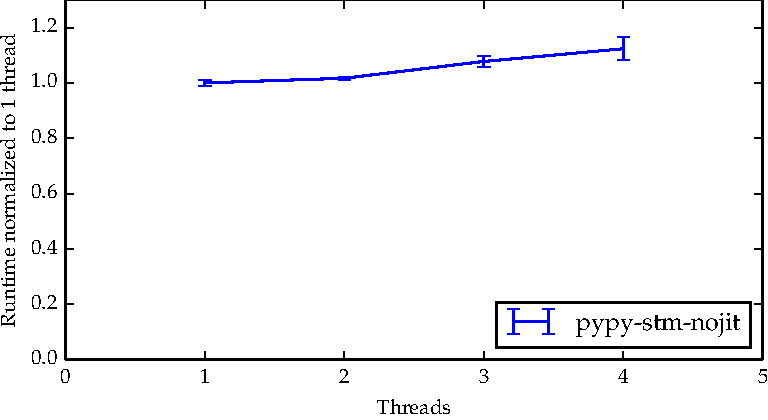
\includegraphics[width=1\columnwidth]{plots/scaling.pdf}
  \caption{Scalability of the STM system\label{fig:scaling}}
\end{figure}


\subsection{Small-Scale Benchmarks\label{sec:performance-bench}}

For the following sections we use a set of six small benchmarks
available on \cite{pypybenchs}:

\begin{itemize}
\item \emph{btree} and \emph{skiplist}, which are both inserting,
  removing, and finding elements in a data structure from multiple
  threads
\item \emph{threadworms}, which simulates worms walking on a grid in
  parallel and checking for collisions with each other
\item \emph{mandelbrot}, \emph{raytrace}, and \emph{richards}, which
  all perform some independent computations in parallel (embarrassingly
  parallel)
\end{itemize}

We use atomic blocks in order to easily synchronise access to shared
data structures in the first three benchmarks. For the embarrassingly
parallel benchmarks, we do not need any explicit synchronisation at
all. These atomic blocks are simulated with a single global lock
when running on top of GIL-supported interpreters. With our STM
system, they map to transactions that will execute optimistically
in parallel.


%%% TODO: if time permits
% \subsection{Overhead Breakdown}

% \remi{do it on a non-jit build (see reason above)}
% \remi{gs:segment prefix overhead is virtually none (maybe instruction cache)}
% \remi{update numbers in pypy/TODO}

% \begin{itemize}
% \item time taken by read \& write barriers
% \item time spent committing \& aborting (maybe with different numbers
%   of threads; maybe split conflict detection and obj sync on commit)
% \item time in GC
% \end{itemize}





\subsection{Non-JIT Benchmarks}
First we run our benchmarks on three different interpreters: CPython
(GIL), and PyPy with STM and with the GIL (both without the JIT). The
results are shown in Figure~\ref{fig:performance-nojit}.

As expected, GIL-supported interpreters do not scale with the number
of threads. They even become slower because of the overhead of
thread-switching and GIL handling (see~\cite{beazley10} for a detailed
analysis).

PyPy using our STM system (\emph{pypy-stm-nojit}) scales in all
benchmarks to a certain degree. It scales best for the embarrassingly
parallel ones and a little less in the others. The reason
for that is that in the former group there are no real, logical
conflicts -- all threads do independent calculations. STM simply
replaces the GIL in those programs. In the latter group,
the threads work on a common data structure and therefore
create much more conflicts, which limits the scalability. Here
we make active use of the STM-supported atomic blocks that
provide a scalable synchronisation mechanism.

Looking at the average overhead from switching from GIL to STM, we see
that it is \remi{$\approx 35.5\%$}. The maximum in richards is
\remi{$63\%$}.

\emph{pypy-stm-nojit} beats \emph{pypy-nojit} already on two threads;
however, it rarely beats CPython's single-thread performance.  For
programs that need concurrency in CPython and that use threads to
achieve this, it also makes sense to look at the overhead induced by
the GIL on multiple threads. From this perspective, the STM
implementation beats CPython's performance in all but two benchmarks.

Since PyPy comes with a JIT to make its overhead compared to CPython
go away, we will now look at how well STM works together with it.

\begin{figure}[h]
  \centering
  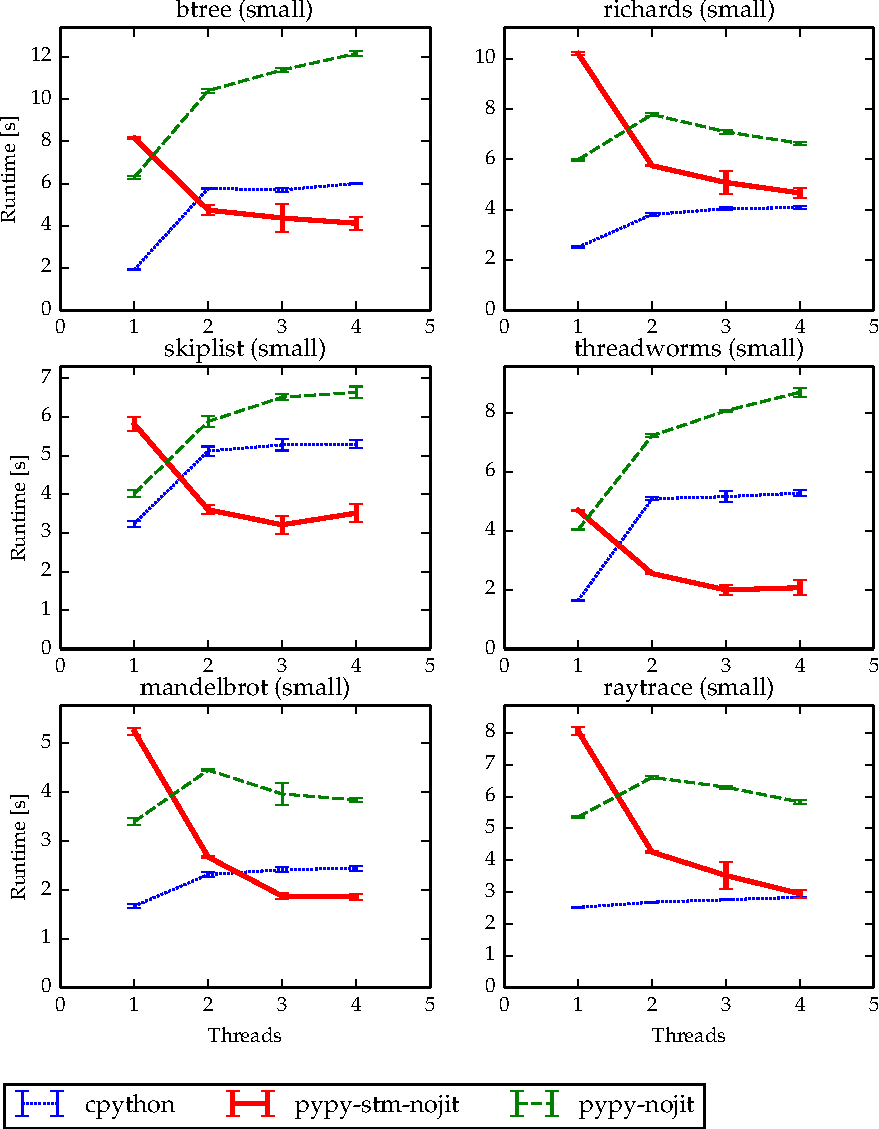
\includegraphics[width=1\columnwidth]{plots/performance_nojit.pdf}
  \caption{Comparing execution time between interpreters without a JIT\label{fig:performance-nojit}}
\end{figure}



\subsection{JIT Benchmarks\label{subsec:jit-benchs}}

We would like to regard enabling the JIT as a simple performance
enhancement, but that is not what happens in reality. First, since the
JIT~\cite{cfbolz09} bases its decision of what to compile on runtime
profiling, running in multiple threads, it may compile different
things in each run because of the non-deterministic thread-scheduling
of the operating system (OS). Second, it is able to remove some
allocations in some cases. Because compilation is already
non-deterministic, so is this allocation-removal. And third, we did
not have enough time to optimise integration with STM so that the JIT
exposes the overhead of STM more by speeding up all the rest.
For these reasons, the following results have to be taken with a grain
of salt.

The speedups from enabling the JIT in these benchmarks range from
$10-50\times$. This is why we had to do without CPython here, since it
would be much further up in the plots. Also, in order to make jitting
code worthwhile, we increased the input size of all benchmarks to get
reasonable execution times.

We also ran these benchmarks on Jython\footnote{version
2.7b1~\cite{webjython}}, an implementation of Python on top of the
Java Virtual Machine (JVM).  Instead of a GIL, this interpreter uses
fine-grained locking for synchronisation. Even though it can use the
JVM's JIT compiler, its performance in these benchmarks is behind
PyPy's by a factor of \remi{$5-10\times$}. Because of that it does not
make sense to include it in this evaluation. In the future, we would
like to do an extensive comparison between the STM approach and
fine-grained locking. It is out of the scope of this paper to do
this thoroughly.

The results are presented in Figure~\ref{fig:performance-jit}. We
see that the performance is much less stable. There is certainly more
work required in this area. The slowdown factor for switching from GIL
to STM ranges around \remi{$1-2.4\times$}, and we beat GIL performance
in half of the benchmarks.

We see that generally, the group of embarrassingly parallel benchmarks scales
best. The other three scale barely or not at all with the number of
threads. The reason for this is likely again the conflicts in the
latter group. Since the JIT accelerates all code but not the STM
overhead, we do more work per transaction. This increases the
likelihood of conflicts between them and therefore limits scalability
even more than in the no-JIT benchmarks.

Overall PyPy needs the JIT in order for its performance to be
competitive with CPython's. It would be interesting to see how using
our STM system in CPython would turn out, but it is a lot of work. On
its own, our system scales well, so we hope to also see that with the
JIT in the future.


\begin{figure}[h]
  \centering
  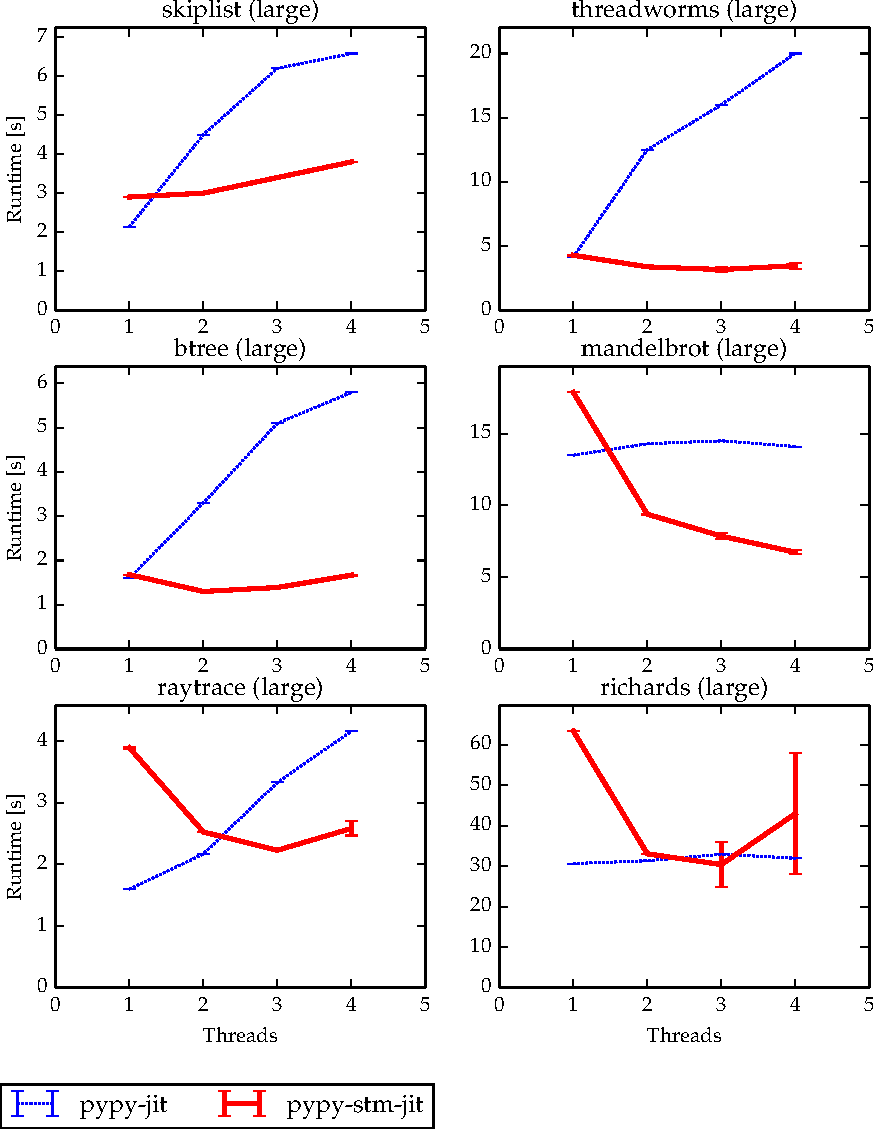
\includegraphics[width=1\columnwidth]{plots/performance.pdf}
  \caption{Comparing execution time between interpreters with JIT\label{fig:performance-jit}}
\end{figure}




\section{Future Work}

\arigo{what else than memory usage goes here?}
\remi{limited scalability; static segmentation?}

We are still working on a number of optimizations in the
implementation.  We want to mention notably that memory usage has not
been optimized so far.  There are several sources of extra memory
requirements in our STM system.  The multiple nurseries add
4~MiB\footnote{Configurable value taken from experience with our
  non-STM reference interpreter.} per segment.  Additionally, the area
used for the read markers uses, per segment, up to 1/16th of the
memory used by the old objects.  With four segments, this adds $25\%$
to the total memory requirements.

One of the most important sources of additional memory usage is the
presence of privatised pages.  It is hard to predict and control.
Right now, if a program creates a large number of privatised pages,
major garbage collections will occur more frequently in the hope of
resharing some of these pages.  More advanced techniques might be
useful.

Overall, early measures seem to show that a four-segment version of
pypy-stm-nojit consumes between 2 and 7 times as much memory as a
plain pypy-nojit.  The high part of this spectrum seems to occur only
if the total memory usage is rather low (less than 20~MiB): it might
simply mean that our approach has a high constant memory usage
overhead.  The low part, i.e.\ a factor 2, can approximately be
attributed to the reasons described above.  It is future work to
investigate in more details.



\section{Related Work}

There have been several attempts at removing the GIL using TM. We
ourselves did a few earlier attempts with more conventional STM
systems~\cite{stmupdate13}. Because of the huge overhead we
encountered, the result was mostly useless on $\le 4$ CPU cores.
Since this could be considered the main operating conditions of
dynamic languages, it was never as useful as we wanted it to be.

Other attempts using HTM~\cite{nicholas06,odaira14,fuad10} show
promising results, especially the very recent~\cite{odaira14} that
examines the current generation of Intel CPUs. However, they did a
simplification by essentially disabling the GC during the
benchmarks. This may be valid for the hand-tuned allocations in their
interpreter. For us the GC is essential, and because it is a moving
GC, it unfortunately touches a lot more memory and thereby reaches the
HTM capacity much faster.  This, and the fact that HTM's capacity
limits do not allow the implementation of arbitrary atomic blocks, let
us to believe that STM is the right choice at the moment.

There are multiple attempts at removing the limits of HTM by means of
\emph{virtualising} HTM~\cite{rajwar05,chung06}. Indeed this may also
be the future direction of our research. So far, some of them depend
on additional hardware features. Or in the case of~\cite{chung06},
they have the assumption that most transactions fit the HTM capacity
and that virtualisation is only a fallback. Our use case, however,
features arbitrarily long transactions, which is why this assumption
first has to be verified in our case.

From the other end, there also have been attempts at lowering the
overhead of STM~\cite{warmhoff13,spear09} especially for a low number
of CPU cores. \cite{spear09} works well for some workloads, in the
case of a dynamic language VM, we have to assume any possible
workload.  \cite{warmhoff13} uses a compile-time approach to select
from multiple optimised STMs. Their partitioned FastLane STM seems to
provide good performance already on two threads using master and
helper threads. It would be interesting to see if its design also
performs well in our use case.

Similarly to us, \cite{martin09} use memory management techniques to
provide isolation between transactions. They focus on providing strong
atomicity between transactional and non-transactional code.  We,
however, use inevitable transactions to provide strong atomicity.
Additionally, while they use page fault handlers to detect conflicts,
we use traditional write barriers. Again, there are only some
superficial similarities between our approach and theirs.


% Similar STMs:
% \begin{itemize}
% \item FastLane: \cite{warmhoff13}
% \item TML: \cite{spear09}
% \item Virtualizing HTM: \cite{rajwar05}
% \item Page-based virtualizing HyTM: \cite{chung06}: page-level conflict
%   detection, otherwise hardware extensions required; assumes most
%   transactions fit HTM capacities (not so true here); COW using page-faults;
%   they assume OS-level access to page-tables (maybe not inherent to their
%   design); eval on simulator; value-based confl detection;

%  (XTM can be
%   implemented either in the OS as part of the virtual memory manager or
%   between underlying TM systems and the OS, like virtual machines;
%   Conflicts for overflowed transactions are tracked at page granularity;
%   XTM-e allows conflict detection at cache line granu-
%   larity, even for overflowed data in virtual memory)
% \item using mmap(): Memory-Mapped Transactions
% \item mem-protected conflict detection: \cite{martin09}
% \end{itemize}


\section{Conclusions}


%% \appendix
%% \section{Appendix Title}

%% This is the text of the appendix, if you need one.

\acks
...

% We recommend abbrvnat bibliography style.

\bibliographystyle{abbrvnat}

% The bibliography should be embedded for final submission.

%%% TODO: fix all citation to follow common format (always page numbers; no 'et al', etc)

\begin{thebibliography}{}
\softraggedright

\bibitem{cfbolz09} Carl Friedrich Bolz, Antonio Cuni, Maciej
  Fijalkowski, and Armin Rigo. 2009. Tracing the meta-level: PyPy's
  tracing JIT compiler.  \emph{In Proceedings of the 4th workshop on the
    Implementation, Compilation, Optimization of Object-Oriented Languages
    and Programming Systems} (ICOOOLPS '09).

\bibitem{kevin10} Kevin Millikin, Florian Schneider. 2010.  A New
  Crankshaft for V8.
  \url{http://blog.chromium.org/2010/12/new-crankshaft-for-v8.html}

\bibitem{ionmonkey} IonMonkey from Mozilla. 2014.
  \url{https://wiki.mozilla.org/IonMonkey/Overview}

\bibitem{wayforward14} Remigius Meier, Armin Rigo. 2014. A Way Forward
  in Parallelising Dynamic Languages. To appear in ICOOOLPS'14.

\bibitem{cpython} CPython. \url{www.python.org}
\bibitem{webjython} The Jython Project, \url{www.jython.org}
\bibitem{ironpython} IronPython. \url{www.ironpython.net}

\bibitem{beazley10} Beazley, David. "Understanding the python gil."
  \emph{PyCON Python Conference}. Atlanta, Georgia. 2010.

\bibitem{harris10} Harris, Tim, James Larus, and Ravi
  Rajwar. "Transactional memory." \emph{Synthesis Lectures on Computer
  Architecture 5.1} (2010): 1-263.

\bibitem{guerraoui08} Guerraoui, Rachid, and Michal Kapalka. "On the
  correctness of transactional memory." \emph{Proceedings of the 13th
    ACM SIGPLAN Symposium on Principles and practice of parallel
    programming.} ACM, 2008.

\bibitem{blundell06} Blundell, Colin, E. Christopher Lewis, and Milo
  Martin. "Unrestricted transactional memory: Supporting I/O and system
  calls within transactions." (2006).
\bibitem{spear08} Spear, Michael F., et al. "Implementing and
  exploiting inevitability in software transactional memory."
  \emph{Parallel Processing, 2008}. ICPP'08. 37th International
  Conference on. IEEE, 2008.

\bibitem{fergus02} Fergus Henderson. 2002. Accurate garbage collection
  in an uncooperative environment. \emph{In Proceedings of the 3rd
    international symposium on Memory management} (ISMM '02).

\bibitem{stmupdate13} Armin Rigo, Remigius Meier. 2013. Update on
  STM. \url{morepypy.blogspot.ch/2013/10/update-on-stm.html}

\bibitem{rajwar05} Rajwar, Ravi, Maurice Herlihy, and Konrad
  Lai. "Virtualizing transactional memory." \emph{Computer
    Architecture}, 2005. ISCA'05. Proceedings. 32nd International
  Symposium on. IEEE, 2005.

\bibitem{chung06} Chung, JaeWoong, et al. "Tradeoffs in transactional
  memory virtualization." \emph{ACM SIGARCH Computer Architecture
  News}. Vol. 34. No. 5. ACM, 2006.

\bibitem{martin09} Martín Abadi, Tim Harris, and Mojtaba
  Mehrara. 2009. Transactional memory with strong atomicity using
  off-the-shelf memory protection hardware. SIGPLAN Not. 44, 4 (February
  2009), 185-196.

\bibitem{pypybenchs} PyPy benchmarks repository. 2014. Revision
  a26f2fb58413. \url{bitbucket.org/pypy/benchmarks}


%%%%%%%%%%%%%%%%%%%%%%%%%%%%%%%%%%%%%%%%%%%%%%%%%%%%%%%%%%%%

% \bibitem{dan07}
%   Dan Grossman. 2007. The transactional memory / garbage collection
%   analogy. \emph{In Proceedings of the 22nd annual ACM SIGPLAN
%     conference on Object-oriented programming systems and
%     applications} (OOPSLA '07).


\bibitem{odaira14}
  Odaira, Rei, Jose G. Castanos, and Hisanobu Tomari.  "Eliminating
  global interpreter locks in Ruby through hardware transactional
  memory."  \emph{Proceedings of the 19th ACM SIGPLAN symposium on
    Principles and practice of parallel programming.} ACM, 2014.

\bibitem{warmhoff13}
  Wamhoff, Jons-Tobias, et al. "FastLane: improving performance of
  software transactional memory for low thread counts."
  \emph{Proceedings of the 18th ACM SIGPLAN symposium on Principles
    and practice of parallel programming.} ACM, 2013.

\bibitem{drago11}
  Dragojević, Aleksandar, et al. "Why STM can be more than a research
  toy." \emph{Communications of the ACM} 54.4 (2011): 70-77.

\bibitem{cascaval08}
  Cascaval, Calin, et al. "Software transactional memory: Why is it
  only a research toy?." \emph{Queue} 6.5 (2008): 40.

\bibitem{nicholas06}
  Nicholas Riley and Craig Zilles. 2006. Hardware transactional memory
  support for lightweight dynamic language evolution. \emph{In
    Companion to the 21st ACM SIGPLAN symposium on Object-oriented
    programming systems, languages, and applications} (OOPSLA
  '06). ACM, New York, NY, USA

\bibitem{fuad10}
  Fuad Tabba. 2010. Adding concurrency in python using a commercial
  processor's hardware transactional memory support. \emph{SIGARCH
  Comput. Archit. News 38}, 5 (April 2010)

% \bibitem{felber07}
%   Felber, Pascal, et al. "Transactifying applications using an open
%   compiler framework." \emph{TRANSACT}, August (2007): 4-6.

% \bibitem{bill06}
%   Bill McCloskey, Feng Zhou, David Gay, and Eric
%   Brewer. 2006. Autolocker: synchronization inference for atomic
%   sections. \emph{In Conference record of the 33rd ACM SIGPLAN-SIGACT
%   symposium on Principles of programming languages (POPL '06)}. ACM,
%   New York, NY, USA

\bibitem{spear09}
  Spear, Michael F., et al. "Transactional mutex locks." \emph{SIGPLAN
    Workshop on Transactional Computing.} 2009.

\bibitem{lamport79}
  Lamport, Leslie. "How to make a multiprocessor computer that
  correctly executes multiprocess programs." \emph{Computers, IEEE
    Transactions} on 100.9 (1979): 690-691.

\bibitem{victor11}
  Victor Pankratius and Ali-Reza Adl-Tabatabai. 2011. A study of
  transactional memory vs. locks in practice. In \emph{Proceedings of
    the twenty-third annual ACM symposium on Parallelism in algorithms
    and architectures} (SPAA '11). ACM, New York, NY, USA

\bibitem{christopher10}
  Christopher J. Rossbach, Owen S. Hofmann, and Emmett
  Witchel. 2010. Is transactional programming actually
  easier?. \emph{SIGPLAN} Not. 45, 5 (January 2010), 47-56.

\bibitem{tim03}
  Tim Harris and Keir Fraser. 2003. Language support for lightweight
  transactions. \emph{In Proceedings of the 18th annual ACM SIGPLAN
    conference on Object-oriented programing, systems, languages, and
    applications} (OOPSLA '03).

\bibitem{tim05}
  Tim Harris, Simon Marlow, Simon Peyton-Jones, and Maurice
  Herlihy. 2005. Composable memory transactions. \emph{In Proceedings
    of the tenth ACM SIGPLAN symposium on Principles and practice of
    parallel programming} (PPoPP '05).

\bibitem{shan08}
  Shan Lu, Soyeon Park, Eunsoo Seo, and Yuanyuan Zhou. 2008. Learning
  from mistakes: a comprehensive study on real world concurrency bug
  characteristics. \emph{SIGARCH Comput. Archit. News} 36, 1 (March 2008),
  329-339.

% \bibitem{leis14}
%   Leis, Viktor, Alfons Kemper, and Thomas Neumann. "Exploiting
%   Hardware Transactional Memory in Main-Memory Databases."
%   \emph{Proc. of ICDE}. 2014.

% \bibitem{biased}
%   Kenneth Russell and David Detlefs. 2006. Eliminating
%   synchronization-related atomic operations with biased locking and
%   bulk rebiasing. \emph{In Proceedings of the 21st annual ACM SIGPLAN
%     conference on Object-oriented programing, systems, languages, and
%     applications} (OOPSLA '06).

\end{thebibliography}


\end{document}
